% -*- TeX-engine: luatex; -*-
\documentclass{article}
\usepackage{ttn}
\usepackage{graphicx}
\usepackage{hyperref}
\usepackage{booktabs}
\usepackage[Ragged, size=footnote, shape=up, alerton]{sidenotesplus}
\usepackage[dvipsnames]{xcolor}
\usepackage{siunitx}
%% 
%%\usepackage[style=authoryear]{biblatex}
%%\addbibresource{notes.bib}
%%
%%
%% \defn takes an optional star and an optional argument.
%% If the optional argument is present, it is used for the marginal note; if the argument is missing, the default is the mandatory argument. if the command is starred, no marginal note is made. 
%% 
\title{The pinhole camera model}
\author{James Geddes}
\date{\today}
%%
\renewcommand{\vec}[1]{\mathbf{#1}}
\begin{document}%\maketitle
\maketitle

\section*{Conversion between camera and world frames}
\begin{marginfigure}
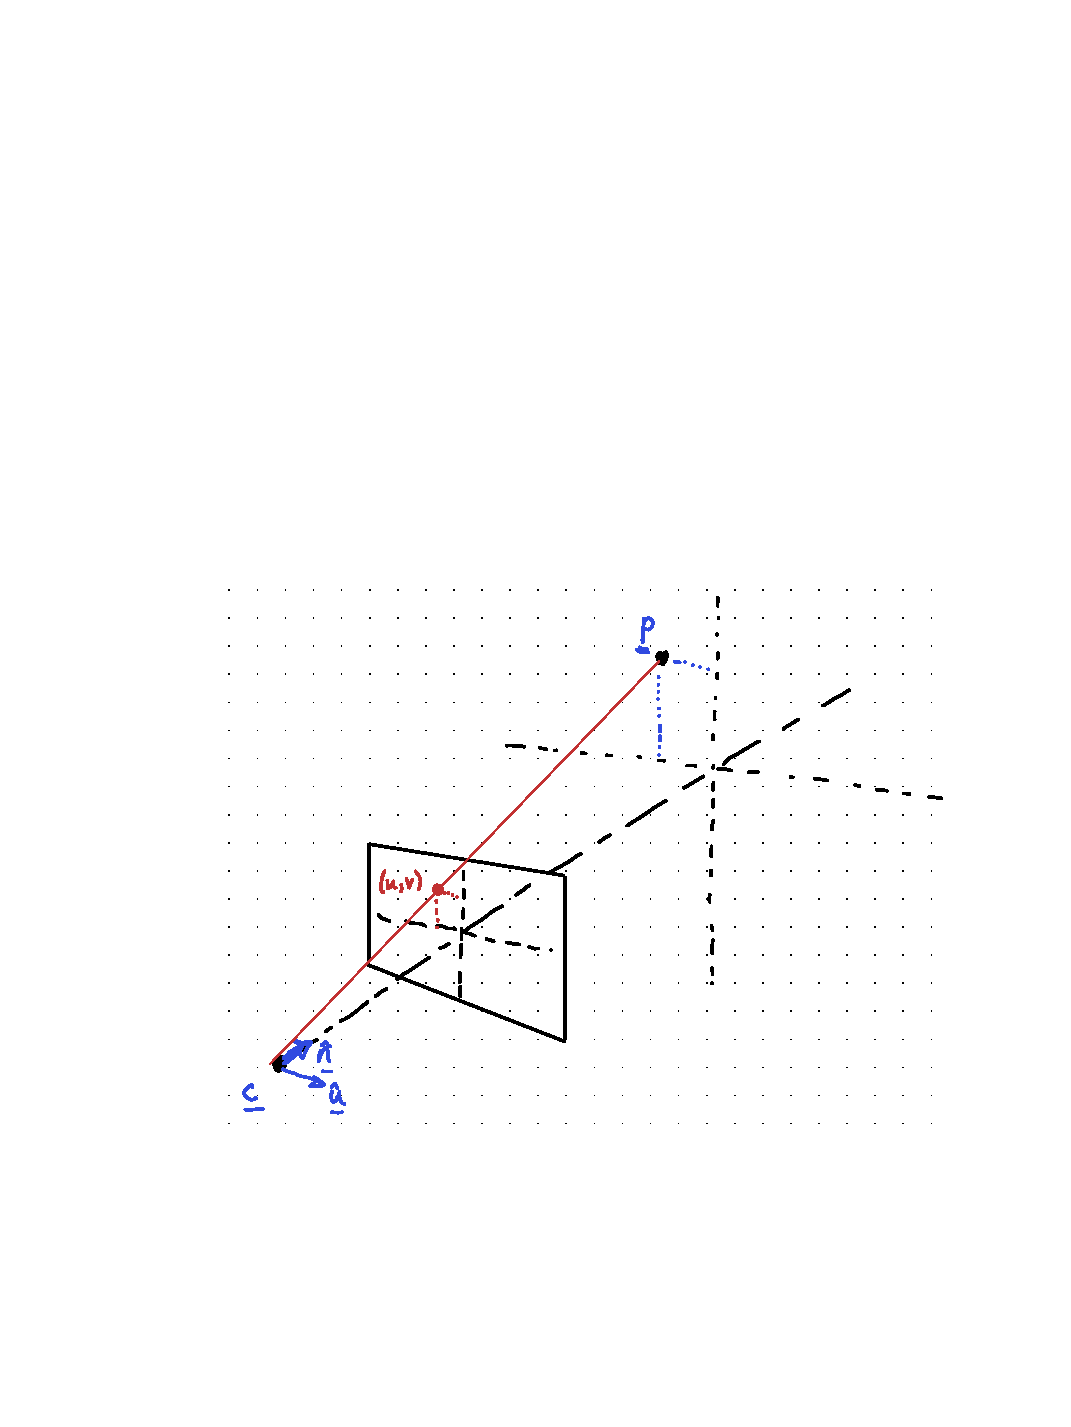
\includegraphics[width=\marginparwidth]{fig1.pdf}
\end{marginfigure}

A camera is defined by: its location, $\vec{c}$; a unit vector,
$\hat{\vec{n}}$, pointing in the direction of view; a unit vector,
$\hat{\vec{u}}$, orthogonal to $\hat{\vec{n}}$ and defining the
``horizontal'' of the image plane; and a ``focal length,'' $f$. It's
convenient to define $\hat{\vec{v}}= \hat{\vec{u}}\times\hat{\vec{n}}$,
a unit vector pointing ``up'' in the camera frame. The focal length
has units of ``pixels per metre'' and is the size, in the camera
frame, of an object of size \qty{1}{\metre} at a distance
of~\qty{1}{\metre} in the world frame.

Coordinates on the image taken by the camera are written $(u,v)$. The
origin is the centre of the image (rather than, as is conventional in
images, the top-left of the image).

The coordinates $(u,v)$ of the image of a point $\vec{p}$ (in the real
world) is determined as follows.
\begin{enumerate}
\item Compute $\vec{x} = \vec{p}-\vec{c}$, the vector from the camera
  to the point;
\item Compute $d = \vec{x}\cdot\hat{\vec{n}}$, the distance from the
  camera to a plane orthogonal to $\hat{\vec{n}}$ containing~$\vec{p}$;
\item Compute $\vec{x}/d - \hat{\vec{n}}$, a vector lying in the above
  plane scaled by the distance to the camera;
\item Project onto the ``image axes,'' and scale to obtain
\begin{equation*}
  \begin{split}
    u &= f \bigl( \vec{x}/d - \hat{\vec{n}} \bigr) \cdot\hat{\vec{u}} \\
      &= (\vec{x}\cdot\hat{\vec{u}})f/d,
  \end{split}
\end{equation*}
  and
\begin{equation*}
  \begin{split}
    v &= (\vec{x}\cdot\hat{\vec{v}})f/d. \\
  \end{split}
\end{equation*}
\end{enumerate}

Conversely, if one starts with a position, $(u, v)$, in the camera's
frame, one obtains a ray in the real world. A ray is a set of points,
$\vec{c}+\lambda \hat{\vec{r}}$, where $\vec{c}$ is a point on the ray
(at the camera's location), and $\lambda\geq 0$ a number. To compute
$\hat{\vec{r}}$: 
\begin{enumerate}
\item An unnormalised ray direction is
  $\vec{r} = \hat{\vec{n}} + (u\vec{u}+v\vec{v})/f$.
\item A normalised ray direction is $\hat{\vec{r}} = \vec{r}/\left|\vec{r}\right|$.
\end{enumerate}

\section*{Ray intersection}

Suppose one has two rays, $\vec{c}_1 + \lambda \vec{r}_1$ and
$\vec{c}_2 + \mu\vec{r}_2$ (where $\vec{r}_1$ and $\vec{r}_2$ are not
necessarily normalised). Their ``approximate intersection'' is the
midpoint on the shortest line joining the two rays. That shortest line
runs from, say, $\vec{p}(s) = \vec{c}_1 + s \vec{r}_1$ to
$\vec{q}(t) = \vec{c}_2 + t \vec{r}_2$ for some $s$ and $t$. Critically,
$\vec{p}(s)-\vec{q}(t)$ is perpendicular to both rays.

Writing $\vec{r} = \vec{c}_1 - \vec{c}_2$, we thus obtain:
\begin{equation}
  \begin{split}
    \vec{r}_1\cdot \bigl( \vec{r} + s\vec{r_1} - t\vec{r_2} \bigr)
    &=0, \qquad\text{and} \\
    \vec{r}_2\cdot \bigl( \vec{r} + s\vec{r_1} - t\vec{r_2} \bigr) &=0,
  \end{split}
\end{equation}
or, rewriting:
\begin{equation}
  \begin{pmatrix}
    \vec{r}_1\cdot\vec{r} \\
    \vec{r}_2\cdot\vec{r} 
  \end{pmatrix} =   
  \begin{pmatrix}
    -\vec{r}_1\cdot\vec{r}_1 & \vec{r}_1\cdot\vec{r}_2 \\
    -\vec{r}_1\cdot\vec{r}_2 & \vec{r}_2\cdot\vec{r}_2 
  \end{pmatrix}
  \begin{pmatrix}
    s \\
    t
  \end{pmatrix}.
\end{equation}
Thus, writing
\begin{equation}
  a = \vec{r}_1\cdot\vec{r}_1,\quad
  b = \vec{r}_1\cdot\vec{r}_2,\quad
  c = \vec{r}_2\cdot\vec{r}_2,\quad
  d = \vec{r}_1\cdot\vec{r},\quad
  e = \vec{r}_2\cdot\vec{r},
\end{equation}
we get
\begin{equation}
  \begin{pmatrix}
    d \\ e
  \end{pmatrix} =   
  \begin{pmatrix}
    -a & b \\
    -b & c
  \end{pmatrix}
  \begin{pmatrix}
    s \\
    t
  \end{pmatrix}.
\end{equation}
Whose solution is:
\begin{equation}
  s = \frac{cd-be}{b^2-ac}\quad\text{and}\quad t = \frac{bd-ae}{b^2-ac}.
\end{equation}


\section*{Euler angles}
Often the camera's orientation is expressed as a rotation matrix,
$\vec{R}$, so that $\hat{\vec{n}} = \vec{R}\hat{\vec{y}}$ (where
$\hat{\vec{y}}$ is the unit vector in the $y$-direction) and
$\hat{\vec{u}}=\vec{R}\hat{\vec{x}}$ (likewise). Both the unit vectors
and the rotation matrix are easy to write down but involve a
constraint. Thus, they are not convenient parametrisations of the
aspect of the camera. The usual alternative is the Euler angles. We
use the following convention, based on the way one imagines that the
camera is physically oriented:
\begin{enumerate}
\item $\alpha$ is the rotation around the $z$-axis (this being the
  principal axis of the tripod). Convention is right-handed, so ``from
  $x$ to $y$;'' that is, the original $\hat{\vec{y}}$ will end up with
  a small $-\hat{\vec{x}}$ component.
\item $\beta$ now rotates about the \emph{new} $x$-axis (corresponding
  to tilting the camera up or down). A positive $\beta$ is upwards. 
\item Finally, $\gamma$ rotates about the resulting $y$-axis
  (corresponding to a change in the ``horizontal,'' relative to the
  camera). A positive $\gamma$ is a clockwise tilt, looking from the
  back of the camera.
\end{enumerate}
(Following Wikipedia, the above convention would be written
$z$-$x'$-$y''$; these are sometimes called Tait-Bryan angles, although
even here there are multiple conventions, depending on the order of
the axes.)

\appendix
\section*{Conversions}
\subsection*{The rotation matrix in terms of the Euler angles}

(Thanks Claude.)
\begin{equation}
  R = \left(
  \begin{matrix}
    \cos\alpha \cos\gamma - \sin\alpha \sin\beta \sin\gamma
    & -\sin\alpha \cos\beta
    & \cos\alpha \sin\gamma + \sin\alpha \sin\beta \cos\gamma \\
    \sin\alpha \cos\gamma + \cos\alpha \sin\beta \sin\gamma
    & \cos\alpha \cos\beta
    & \sin\alpha \sin\gamma - \cos\alpha \sin\beta \cos\gamma \\
    -\cos\beta \sin\gamma
    & \sin\beta
    & \cos\beta \cos\gamma
  \end{matrix}
  \right)
\end{equation}

In terms of the individual rotations,
\begin{equation}
  R = R_z(\alpha) R_x(\beta) R_y(\gamma), 
\end{equation}
where
\begin{equation}
  \begin{split}
    R_z(\alpha) &= 
    \left(\begin{matrix}
      \cos\alpha & -\sin\alpha & 0 \\
      \sin\alpha & \cos\alpha & 0 \\
      0 & 0 & 1
    \end{matrix}\right), \\
    R_x(\beta) &= 
    \left(\begin{matrix}
      1 & 0 & 0 \\
      0 & \cos\beta & -\sin\beta \\
      0 & \sin\beta & \cos\beta 
    \end{matrix}\right), \\
    R_y(\gamma) &= 
    \left(\begin{matrix}
      \cos\gamma & 0 & \sin\gamma \\
      0 & 1 & 0 \\
      -\sin\gamma & 0 & \cos\gamma 
    \end{matrix}\right).
  \end{split}
\end{equation}

\subsection*{The unit normals in terms of the rotation matrix}

In fact, the unit normals (to the rotated camera), expressed in the
world coordinate system, are just the columns of the rotation matrix.

\subsection*{The Euler angles from the rotration matrix}

Writing $R_{ij}$ for the $i$th row and $j$th column, indexed from zero:

\begin{equation}
  \begin{split}
    \alpha &= \arctan(-R_{01}/ R_{11}) \\
    \beta  &= \arcsin(R_{21}) \\
    \gamma &= \arctan(-R_{20}/ R_{22})
  \end{split}
\end{equation}

In practice, instead of $\arctan(-y/x)$ in the above we use the
function ``\texttt{atan2(y,x)}'' which ensures that the angle is in
the correct range. (See Wikipedia.)

\end{document}
